\documentclass[%
  reprint,
  superscriptaddress,
  showpacs,
  showkeys,
  amsmath,amssymb,
  pra,
  longbibliography,
  floatfix,
  x11names
]{revtex4-2}

\usepackage{amsmath}
\usepackage{amssymb}
\usepackage{amsthm}
\usepackage{bm} % bold math
\usepackage{graphicx}
\usepackage{tikz}
\usetikzlibrary{decorations.markings,lindenmayersystems}
\usepackage{pgfplots}
\pgfplotsset{compat=1.18}
\usepackage{orcidlink}
\usepackage{hyperref}

% --- DEFINITIONS FOR FIGURES (MUST BE IN PREAMBLE) ---

% Configuration parameters for Menger Sponge
\definecolor{cubeface1}{RGB}{180,180,180}  % Right face
\definecolor{cubeface2}{RGB}{220,220,220}  % Top face
\definecolor{cubeface3}{RGB}{140,140,140}  % Front face
\definecolor{cubeedge}{RGB}{80,80,80}      % Edge color

\newcommand\mengersponge[2][]{
    \pgfkeys{
        /menger/.cd,
        draw edges/.initial=true,
        edge width/.initial=0.1pt,
        .unknown/.style={\pgfkeyscurrentname/.style={#1}}
    }
    \pgfkeys{/menger/.cd, #1}

    \pgfmathsetmacro\level{int(#2 - 1)}
    \ifnum \level = 0 \relax
        \mengercube
    \else
        \begin{scope}[scale=0.333333]
            \foreach \x in {-2,0,2} {
                \foreach \y in {-2,0,2} {
                    \foreach \z in {-2,0,2} {
                        \pgfmathsetmacro{\skipthis}{
                            (\x==0 && \y==0) || (\x==0 && \z==0) || (\y==0 && \z==0) ? 1 : 0
                        }
                        \ifnum\skipthis=0
                            \begin{scope}[shift={(\x,\y,\z)}]
                                \mengersponge[#1]{\level}
                            \end{scope}
                        \fi
                    }
                }
            }
        \end{scope}
    \fi
}

\newcommand\mengercube{
    \filldraw[
        fill=cubeface1,
        draw=cubeedge,
        line width=\pgfkeysvalueof{/menger/edge width}
    ] (1,1,1) -- (1,1,-1) -- (1,-1,-1) -- (1,-1,1) -- cycle;
    \filldraw[
        fill=cubeface2,
        draw=cubeedge,
        line width=\pgfkeysvalueof{/menger/edge width}
    ] (1,1,1) -- (1,1,-1) -- (-1,1,-1) -- (-1,1,1) -- cycle;
    \filldraw[
        fill=cubeface3,
        draw=cubeedge,
        line width=\pgfkeysvalueof{/menger/edge width}
    ] (1,1,1) -- (1,-1,1) -- (-1,-1,1) -- (-1,1,1) -- cycle;
}

% Koch curve
\pgfdeclarelindenmayersystem{Koch curve}{
  \rule{F -> F+F--F+F}
}

% Cantor set
\pgfdeclarelindenmayersystem{Cantor set}{
  \rule{F -> FfF}
  \rule{f -> fff}
}
% --- END OF FIGURE DEFINITIONS ---

\begin{document}

\title{Anti-Gravity from Vacancies in Fractal Space-Time: The Case of a Menger Sponge}

\author{Karl Svozil\,\orcidlink{0000-0001-6554-2802}}
\email{karl.svozil@tuwien.ac.at}
\homepage{http://tph.tuwien.ac.at/~svozil}
\affiliation{Institute for Theoretical Physics, TU Wien, Wiedner Hauptstrasse 8-10/136, 1040 Vienna, Austria}

\date{\today}

\begin{abstract}
We investigate the gravitational properties of a spacetime characterized by a fractal distribution of vacancies, modeled via the Menger Sponge. Treating the fractal structure within a coarse-grained ``effective medium'' description, we construct an effective density profile for a localized vacancy-dominated region and, under the assumption of spherical symmetry, model the corresponding exterior geometry. By integrating out the density deficit relative to a uniform background substratum, we obtain an effective mass parameter that is negative when vacancies dominate, leading to an exterior metric formally equivalent to the negative-mass Schwarzschild solution. In contrast to defect configurations that modify the angular structure of space, a purely density-deficit model leaves the manifold topology intact while still implying a repulsive potential for test particles in the Newtonian limit. We analyze the resulting geodesic motion, discuss the violations of energy conditions required by the effective density profile, and interpret such vacancy-rich regions as emergent repulsive centers within a ponderable background, while emphasizing the phenomenological nature of the construction.
\end{abstract}

\keywords{fractal gravity, anti-gravity, Menger sponge, embedded observers}

\maketitle

\section{Introduction}
\label{sec:intro}

The description of spacetime as a smooth continuum is a central postulate of general relativity (GR). However, several approaches to quantum gravity and discrete spacetime suggest that at microscopic scales spacetime may possess a nontrivial microstructure, possibly with scale-dependent effective dimensionality or fractal properties~\cite{Ambjorn2012_review,barkley-2019}. A key question in such scenarios is how the geometric and dynamical properties of this microstructure manifest to observers who only probe macroscopic, coarse-grained scales.

In parallel, the longstanding analogy between gravity and continuum mechanics has shown that defects in solids---such as dislocations and disclinations---can be described geometrically using Riemann--Cartan or related formalisms~\cite{Kroner-1958,kroner-1990,kleinert-2004,zaanen-2022}. In these models, added or removed material, or changes in the local bonding structure, are encoded in effective curvature and torsion. This viewpoint resonates with Einstein's re-interpretation of the ``ether'' as the geometric spacetime metric~\cite{einstein-aether-en} and with Sakharov's idea of induced gravity, where gravitational dynamics emerge from the elastic response of quantum vacuum fluctuations~\cite{Sakharov-67}.

In this paper, we explore a phenomenological model in which spacetime is endowed with a fractal density of ``vacancies'': regions where an underlying ponderable substratum is absent or rarefied. As a concrete prototype, we use the Menger Sponge, whose non-integer Hausdorff dimension and vanishing volume in the infinite-iteration limit provide a controlled example of a vacancy-dominated configuration embedded in a three-dimensional continuum. Within a coarse-grained, effective-medium perspective, we ask how such a vacancy distribution would appear gravitationally to an observer who only probes length scales large compared to the microscopic structure.

Our strategy is as follows. We assume a uniform background substratum with energy density $\rho_0>0$ and consider a spherically symmetric region in which this substratum has been removed in a fractal, Menger-sponge-like way. We then define an \emph{effective} mass density as the deviation from the background density and integrate this over the defect region to obtain an effective total mass $M_{\text{eff}}$ as seen from outside. In the vacancy-dominated regime, $M_{\text{eff}}$ is negative. By Birkhoff's theorem, the exterior geometry for $r>\mathcal{R}$ is then described by a Schwarzschild metric with mass parameter $M_{\text{eff}}<0$, i.e., by the well-known negative-mass Schwarzschild solution~\cite{bondi-1957}.

We reinterpret this negative mass in terms of a dimensionless defect-strength parameter $S$, constructed from the imbalance between vacancies and interstitials, together with a characteristic microscopic scale $L$. This yields a relation of the form $2M_{\text{eff}} = SL$, which may be viewed as a coarse-grained effective-medium analogue of the standard Schwarzschild mass parameter. We then analyze geodesic motion in the resulting metric and show explicitly that for $S<0$ the free-fall acceleration of test bodies is repulsive. We emphasize throughout that we do not derive a new solution of Einstein's equations from a specified microscopic stress-energy tensor; rather, we provide a phenomenological mapping between a fractal vacancy distribution in a ponderable background and the classical negative-mass Schwarzschild geometry.

The paper is organized as follows. In Sec.~\ref{sec:quant} we introduce the Menger Sponge as a prototype for a vacancy-dominated microstructure and develop an effective-medium model connecting the vacancy density to an effective negative mass parameter. In Sec.~\ref{sec:ricci} we discuss the vacuum character of the exterior spacetime. Section~\ref{sec:geodesic} analyzes geodesic motion, deriving the repulsive free-fall acceleration and distinguishing our density-deficit mechanism from topological defects. Section~\ref{sec:energy} addresses the associated energy-condition and stability issues. We conclude in Sec.~\ref{sec:discuss} with a summary and outlook.


\section{Effective-medium model for fractal vacancies}
\label{sec:quant}

\subsection{Fractal density profile and vacancy-dominated limit}

To model a vacancy-dominated region of spacetime, we utilize the Menger Sponge~\cite{Menger1926a_reprint,Edgar_ClassicsOnFractals}. This fractal is constructed by starting with a unit cube, dividing it into 27 sub-cubes, and removing the central cube and the six cubes at the center of each face. This process is iterated ad infinitum. The resulting set is a universal curve with Hausdorff dimension $D = \ln 20 / \ln 3 \approx 2.73$ and vanishing Lebesgue measure (volume) in the limit.

\begin{figure}[ht]
\centering
\resizebox{.36\textwidth}{!}{
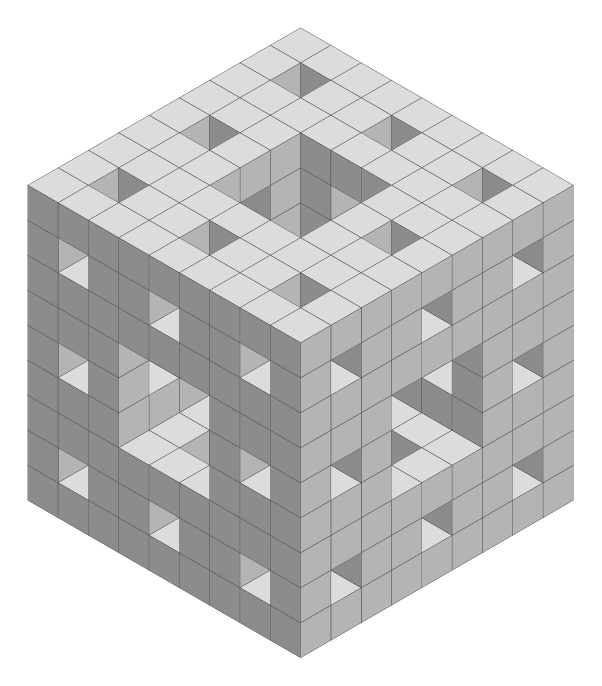
\begin{tikzpicture}[
    x={(0.866cm,-0.5cm)},
    y={(0cm,1cm)},
    z={(-0.866cm,-0.5cm)},
    scale=2
]
    \mengersponge{3}
\end{tikzpicture}
}
\caption{The Menger Sponge at the third iteration. In our model, this represents the distribution of the ponderable substratum, with the transparent regions representing vacancies where the effective density is negative relative to the background.}
\label{fig:menger}
\end{figure}

We consider a spherically symmetric region of radius $\mathcal{R}$ cut out of an otherwise uniform background substratum with energy density $\rho_0>0$.
Within this region, the substratum is arranged in a Menger-sponge-like fashion (Fig.~\ref{fig:menger}).
We emphasize that the exact Menger-sponge geometry is not spherically symmetric; our use of a spherically symmetric effective density profile is a coarse-grained idealization
appropriate for observers probing scales large compared to the elementary cube size. For a fractal set with Hausdorff dimension $D<3$, the mass $M_{\text{frac}}(r)$
of substratum contained within a radius $r\le \mathcal{R}$ scales as
\begin{equation}
M_{\text{frac}}(r) \propto r^D,
\end{equation}
so that the average density measured at scale $r$ behaves as
\begin{equation}
\bar{\rho}_{\text{frac}}(r) = \frac{M_{\text{frac}}(r)}{\frac{4\pi}{3} r^3}
\;\propto\;
r^{-(3-D)}.
\label{eq:scaling}
\end{equation}
In the limit of an infinite-iteration Menger sponge, the retained volume fraction tends to zero while $D<3$ remains fixed, so that the actual amount of substratum present inside $\mathcal{R}$ becomes negligible compared to the background expectation.

To describe the gravitational effect of this configuration, we adopt a background-subtracted, effective-medium perspective: we treat only deviations from the uniform background density $\rho_0$ as sources of the effective gravitational field, in analogy with homogenization methods in condensed matter and electrostatics. Accordingly, we define an effective density
\begin{equation}
\rho_{\text{eff}}(r) = \rho_{\text{frac}}(r) - \rho_0,
\label{eq:rho_eff_def}
\end{equation}
where $\rho_{\text{frac}}(r)$ is the coarse-grained density associated with the fractal substratum. In a full general-relativistic treatment, a uniform background density $\rho_0$ would contribute to a cosmological term rather than to a localized mass.
Here we focus on localized deviations from this background and interpret $\rho_{\text{eff}}$ as the relevant source for the \emph{relative} gravitational field produced by the defect region.
This step is in the spirit of Newtonian potential theory and homogenization: we are not attempting a full cosmological solution with the absolute background density $\rho_0$, but rather isolating the local, defect-induced field relative to that background.

In the vacancy-dominated regime, and for a sufficiently high iteration of the Menger construction, the fractal contribution $\rho_{\text{frac}}$ becomes small compared to $\rho_0$ inside the region $r\le \mathcal{R}$. To leading order we then have
\begin{equation}
\rho_{\text{eff}}(r) \simeq -\rho_0 \quad \text{for } r\le\mathcal{R},
\qquad
\rho_{\text{eff}}(r) \simeq 0 \quad \text{for } r>\mathcal{R},
\end{equation}
corresponding to an approximately empty spherical cavity in an otherwise uniform substratum. For a finite-iteration Menger sponge with Hausdorff dimension $D<3$, the residual substratum contributes a subleading positive mass term of order $\mathcal{R}^D$, so that the total effective mass is
\begin{equation}
M_{\text{eff}}
= \int_0^{\mathcal{R}} 4\pi r'^2 \rho_{\text{eff}}(r') \, dr'
= -\frac{4\pi}{3} \rho_0 \mathcal{R}^3 + \mathcal{O}(\mathcal{R}^D).
\label{eq:Meff}
\end{equation}
In the vacancy-dominated regime and for sufficiently large $\mathcal{R}$, the leading term controls the sign, and $M_{\text{eff}}<0$. Thus, from the point of view of an exterior observer who cannot resolve the internal fractal structure, the defect region behaves as an effective negative-mass source of magnitude $|M_{\text{eff}}| \sim \rho_0 \mathcal{R}^3$.

\subsection{Connection to a defect-strength parameter}
\label{sec:defect-source}

We now relate this effective mass to a dimensionless defect-strength parameter that quantifies the imbalance between interstitials (added ``stuff'') and vacancies (removed ``stuff'') at the microscopic level. As in the original phenomenological construction, we introduce dimensionless volume fractions
\begin{equation}
N_i,\,N_v \in [0,1],
\end{equation}
representing, respectively, the fractional abundance of interstitials and vacancies relative to some reference density. We then define the net defect strength
\begin{equation}
S = N_i - N_v.
\end{equation}
By construction, $S>0$ when added material dominates, $S<0$ when vacancies dominate, and $S=0$ for a defect-free reference configuration.

For a Menger-sponge-like configuration at iteration level $n$, the retained volume fraction of substratum is $(20/27)^n$, implying a vacancy fraction
\begin{equation}
v_n = 1 - \left(\frac{20}{27}\right)^n.
\end{equation}
In a coarse-grained description at scales large compared to the elementary cell, it is natural to approximate the local effective density inside the defect region as
\begin{equation}
\rho_{\text{eff}} \simeq (N_i - N_v)\,\rho_0 = S \rho_0,
\end{equation}
so that a pure vacancy configuration with $N_i \approx 0$ and $N_v\approx 1$ has $\rho_{\text{eff}} \approx -\rho_0$, in agreement with Eq.~\eqref{eq:Meff}.

To connect to the Schwarzschild mass parameter, we introduce a characteristic microscopic length scale $L$ (e.g., the initial cube side length or lattice spacing) and write the effective source parameter as
\begin{equation}
\beta := 2 M_{\text{eff}}.
\end{equation}
Dimensional analysis then suggests a relation of the form
\begin{equation}
\beta = S L,
\label{eq:beta_SL}
\end{equation}
where the proportionality constant has been absorbed into the definition of $L$ and of the coarse-grained $S$. This recovers, in the vacancy-dominated limit, the phenomenological ansatz $2M = SL$ of the original model, but now interpreted as the leading contribution of the background-subtracted effective density integrated over the defect volume.

\subsection{Exterior metric as reparameterized Schwarzschild}
\label{2025-menger-gmld}

Outside the defect region ($r>\mathcal{R}$) the effective density vanishes, $\rho_{\text{eff}}=0$, and the spacetime is locally indistinguishable from the unperturbed background. Assuming that the background cosmological contribution associated with $\rho_0$ has been absorbed into a large-scale cosmological constant, the \emph{local} gravitational field of the defect is determined by the effective mass $M_{\text{eff}}$ defined in Eq.~\eqref{eq:Meff}. By Birkhoff's theorem, the most general spherically symmetric vacuum solution of the Einstein equations in this region is the Schwarzschild metric with mass parameter $M_{\text{eff}}$.

For reference, in geometrized units ($G=c=1$) the Schwarzschild line element reads
\begin{equation}
g_{\mu\nu} = \text{diag}\left[-\left(1 - \frac{2M}{r}\right), \left(1 - \frac{2M}{r}\right)^{-1}, r^2, r^2 \sin^2 \theta\right].
\label{eq:schwarzschild}
\end{equation}
Identifying $M$ with $M_{\text{eff}}$ and using Eq.~\eqref{eq:beta_SL}, we may write
\begin{equation}
2M = \beta = SL.
\end{equation}
Implementing this identification amounts to the substitution
\begin{equation}
2M \longrightarrow \beta = SL
\end{equation}
in Eq.~\eqref{eq:schwarzschild}, yielding the effective metric
\begin{equation}
g_{\mu\nu} = \text{diag}\left[-\left(1 - \frac{\beta}{r}\right), \left(1 - \frac{\beta}{r}\right)^{-1}, r^2, r^2 \sin^2 \theta\right].
\label{eq:defect_metric}
\end{equation}
This is \emph{exactly} the Schwarzschild solution with mass parameter
\begin{equation}
2M = \beta = SL, \qquad M = \frac{1}{2} SL.
\end{equation}
No new solution of Einstein's equations is thereby obtained; rather, the mass parameter $M$ is reinterpreted as arising from an effective defect strength $S$ and a microscopic scale $L$ via the effective-medium construction of Sec.~\ref{sec:defect-source}.

The sign of $S$ is crucial:

\begin{itemize}
\item For $S > 0$ (interstitial-dominated), $\beta>0$ and the metric coincides with the standard Schwarzschild spacetime of a positive mass $M>0$, with an event horizon at $r=2M=\beta>0$.
\item For $S < 0$ (vacancy-dominated), $\beta<0$ and the metric corresponds to the exterior geometry of a \emph{negative} mass~\cite{bondi-1957}. In this case $1-\beta/r = 1+|\beta|/r$ never vanishes for $r>0$, so there is no event horizon; the coordinate singularity at $r=2M>0$ present in the usual Schwarzschild solution is absent, while the curvature singularity at $r=0$ remains.
\end{itemize}

In what follows we refer to these two cases as the attractive and repulsive regimes, respectively, emphasizing that this distinction is entirely encoded in the sign of $\beta = SL$. We stress that our construction is phenomenological: it does not derive the Schwarzschild geometry from a specific microscopic stress-energy tensor built from a Menger-sponge microstructure, but rather provides an effective-medium motivation for the identification $2M=SL$ used to reinterpret the standard negative-mass Schwarzschild solution in terms of fractal vacancies.



\section{Ricci Scalar and Vacuum Character}
\label{sec:ricci}

The Ricci scalar \(R\) is related to the trace of the stress-energy tensor \(T\) via the trace of Einstein's equations (with \(\Lambda=0\)),
\begin{equation}
R = -8\pi T.
\end{equation}
Calculating \(R\) for our metric~\eqref{eq:defect_metric} allows us to characterize the spacetime as vacuum or non-vacuum.

As emphasized in Sec.~\ref{2025-menger-gmld}, the metric~\eqref{eq:defect_metric} is simply the Schwarzschild solution with the identification \(2M=\beta\). The Schwarzschild metric is by construction a vacuum solution of the Einstein field equations for all \(r>0\):
\begin{equation}
R_{\mu\nu} = 0 \quad \text{for} \quad r>0,
\end{equation}
irrespective of the numerical value or sign of \(M\). Consequently,
\begin{equation}
R = g^{\mu\nu} R_{\mu\nu} = 0 \quad \text{for} \quad r>0.
\end{equation}
The exterior spacetime is therefore a vacuum region in which the curvature is entirely encoded in the Weyl tensor (tidal fields), with matter content localized at \(r=0\) in the form of a point mass (positive or negative).

This serves as a consistency check that, given our phenomenological identification \(2M = SL\), the resulting geometry is a legitimate vacuum solution of Einstein's equations outside the source. It does \emph{not} constitute a derivation of this geometry from a specific microscopic defect-based stress-energy tensor. Our model remains phenomenological in that respect.

\section{Geodesic Motion and Repulsion}
\label{sec:geodesic}

To decide whether the effective gravitational field is attractive or repulsive, one must examine the motion of test particles. The simplest and most physical test is to study radial timelike geodesics in the metric~\eqref{eq:defect_metric} and determine the sign of their radial acceleration.

\subsection{Proper Acceleration of Static Observers}

For reference, consider first a static observer at fixed spatial coordinates \((r,\theta,\phi)\). The worldline is
\[
x^\mu(\tau) = (t(\tau), r, \theta, \phi),
\]
with four-velocity \(u^\mu = (u^t,0,0,0)\). Normalization \(g_{\mu\nu}u^\mu u^\nu = -1\) gives
\begin{equation}
(u^t)^2 = \frac{1}{1-\beta/r}.
\end{equation}
The four-acceleration of this static observer is
\begin{equation}
a^\mu = u^\nu \nabla_\nu u^\mu = \Gamma^\mu_{\nu\lambda} u^\nu u^\lambda.
\end{equation}
Only the \(tt\) component contributes to the radial part,
\begin{equation}
a^r = \Gamma^r_{tt} (u^t)^2.
\end{equation}
For the metric~\eqref{eq:defect_metric},
\begin{equation}
g_{tt} = -F,\quad g_{rr} = F^{-1},\quad F(r) = 1 - \frac{\beta}{r},
\end{equation}
one finds
\begin{align}
\Gamma^r_{tt}
&= \frac{1}{2} g^{rr} \left(-\partial_r g_{tt}\right)
= \frac{1}{2} F \, \partial_r F
= \frac{1}{2} F \frac{\beta}{r^2},\\
a^r &= \Gamma^r_{tt}(u^t)^2
= \frac{1}{2} F \frac{\beta}{r^2} \frac{1}{F}
= \frac{\beta}{2r^2}.
\end{align}
Thus the proper radial acceleration required to hold a static position is
\begin{equation}
a^r = \frac{\beta}{2r^2}.
\end{equation}
For \(\beta>0\) this acceleration points outward, meaning a static observer must accelerate upward to resist inward gravitational pull, as in the usual Schwarzschild case. For \(\beta<0\) the sign reverses. However, this describes the acceleration of non-geodesic worldlines maintained in place by some non-gravitational force.

\subsection{Free-Fall Geodesics: Attraction vs.\ Repulsion}

The unambiguous probe of attraction or repulsion is the acceleration of freely falling (geodesic) test particles. For radial timelike geodesics, the line element reduces to
\begin{equation}
ds^2 = -\left(1-\frac{\beta}{r}\right) dt^2
+ \left(1-\frac{\beta}{r}\right)^{-1} dr^2.
\end{equation}
Conservation of energy along the geodesic yields a first integral:
\begin{equation}
E = \left(1-\frac{\beta}{r}\right)\frac{dt}{d\tau},
\label{eq:energy}
\end{equation}
where \(\tau\) is proper time and \(E\) is a constant. Using normalization \(u^\mu u_\mu=-1\) and Eq.~\eqref{eq:energy}, one finds for radial motion
\begin{equation}
\left(\frac{dr}{d\tau}\right)^2 = E^2 - \left(1-\frac{\beta}{r}\right).
\end{equation}
Consider a particle released from rest at radius \(r=r_0\), i.e., with initial condition \((dr/d\tau)|_{\tau=0}=0\). Then
\begin{equation}
E^2 = 1-\frac{\beta}{r_0},
\end{equation}
and near \(\tau=0\) one may expand to find the second derivative of \(r\):
\begin{equation}
\left.\frac{d^2 r}{d\tau^2}\right|_{\tau=0}
= -\frac{\beta}{2 r_0^2}.
\end{equation}
This result is analogous to the Newtonian expression with \(\beta=2M\).

The sign is now decisive:
\begin{itemize}
\item For \(S>0\) (\(\beta>0\)), \(\ddot{r}|_0 = -\beta/(2r_0^2)<0\): the particle accelerates inward; the field is attractive.
\item For \(S<0\) (\(\beta<0\)), \(\ddot{r}|_0 = -\beta/(2r_0^2)>0\): the particle accelerates outward; the field is repulsive.
\end{itemize}
Thus, when vacancies dominate (\(N_v > N_i\), hence \(S<0\)), the effective metric~\eqref{eq:defect_metric} describes matter-matter repulsion in the sense of free-fall geodesics. This matches the qualitative picture of vacancies creating intrinsic ``shortcuts'', and it is fully equivalent, at the level of the exterior geometry, to the well-known negative-mass Schwarzschild solution~\cite{bondi-1957}.

\subsection{Topological versus density defects}

It is important to distinguish the mechanism considered here from standard topological defects in solids and in gravitational analogues. In the Volterra process, for example, removing a wedge of material from an elastic medium and gluing the faces results in a cone with a deficit angle. The corresponding geometry has nontrivial topology and positive curvature concentrated along the defect line, and in the gravitational context it is analogous to a cosmic string: test particles experience an effectively attractive interaction associated with the conical singularity.

By contrast, the vacancy-dominated configuration studied in this work does not remove a wedge of the manifold or introduce a nontrivial topology. Instead, it removes \emph{density} from a background substratum within a topologically trivial spherical region. In the Newtonian limit, the gravitational potential is sourced by the sign of the effective mass density: a local deficit relative to the background, encoded in $\rho_{\text{eff}}<0$, acts as a repulsive center for test bodies, as reflected in the outward acceleration for $S<0$ derived in Sec.~\ref{sec:geodesic}. The fractal Menger-sponge structure allows this ``hole'' to be distributed over a finite volume $\mathcal{R}$ while maintaining a smooth manifold for $r>0$, thereby avoiding the conical singularities characteristic of wedge-type defects.

A full dynamical analysis of the stability of such vacancy-induced negative-mass regions would require a microscopic model of the substratum and its coupling to matter fields. Within the present effective-medium framework, we simply treat the vacancy distribution as defining a fixed background configuration with an associated effective mass parameter $M_{\text{eff}}<0$, and we restrict attention to the resulting geodesic motion of test particles in the corresponding exterior Schwarzschild geometry.



\section{Energy Conditions and Exotic Matter}
\label{sec:energy}

Energy conditions are criteria imposed on the stress-energy tensor \(T_{\mu\nu}\) to capture the idea of physically reasonable matter. They constrain combinations such as \(T_{\mu\nu}u^\mu u^\nu\) (energy density) and its variants for null vectors. We briefly review how these conditions apply to our defect-reinterpreted Schwarzschild metric.

\subsection{Vacuum Exterior ($r > 0$)}

As established in Sec.~\ref{sec:ricci}, the spacetime described by Eq.~\eqref{eq:defect_metric} is a vacuum solution for all \(r>0\), in the strict GR sense:
\begin{equation}
T_{\mu\nu} = 0 \quad (r>0).
\end{equation}
All local energy conditions are then trivially satisfied in the vacuum region, e.g.,
\begin{equation}
T_{\mu\nu} k^\mu k^\nu = 0 \ge 0
\end{equation}
for any null vector \(k^\mu\) (Null Energy Condition), and similarly for timelike vectors. The vacuum itself is not exotic; the exoticity, if any, must be localized at the source.

\subsection{Strong Energy Condition and Repulsion}

The Strong Energy Condition (SEC) can be recast geometrically through Einstein's equations as
\begin{equation}
R_{\mu\nu}u^\mu u^\nu \ge 0
\end{equation}
for any timelike vector \(u^\mu\). Combined with the Raychaudhuri equation, this condition ensures that gravity is, on average, attractive: timelike geodesic congruences tend to focus.

In our case, \(R_{\mu\nu}=0\) for \(r>0\), so
\begin{equation}
R_{\mu\nu}u^\mu u^\nu = 0.
\end{equation}
The vacuum region therefore \emph{saturates} the SEC: it neither contributes to focusing nor to defocusing via the Ricci tensor. All gravitational effects in the vacuum arise from the Weyl tensor (tidal fields), not from local matter content.

The global character of the field (attractive vs.\ repulsive) is encoded in the sign of the mass parameter \(M=\beta/2\). For \(M>0\) we have the usual inward attraction, while for \(M<0\) we have outward repulsion as shown in Sec.~\ref{sec:geodesic}. This difference originates in the effective source at \(r=0\).

\subsection{Nature of the Source at the Origin}

The exterior geometry of Eq.~\eqref{eq:defect_metric} can be thought of as produced by a point-like source at \(r=0\) with total gravitational mass
\begin{equation}
M = \frac{1}{2} SL.
\end{equation}
The sign of \(S\) determines whether this mass is positive or negative.

\begin{itemize}
\item \textbf{Attractive regime (\(S>0\)):} The source has positive mass and can in principle be modeled by conventional matter distributions satisfying the usual energy conditions in an appropriate limit.
\item \textbf{Repulsive regime (\(S<0\)):} The source must have negative mass and therefore correspond to exotic matter, violating the averaged forms of the energy conditions. As emphasized long ago by Bondi~\cite{bondi-1957}, such negative-mass sources are associated with run-away instabilities (e.g., in a positive/negative mass pair) and other conceptual issues.
\end{itemize}

Our identification of \(M\) with a defect parameter \(S\) does not eliminate these fundamental problems; it merely reinterprets the negative mass in terms of an effective vacancy-dominated region. From the standpoint of classical GR, the repulsive model still requires an exotic source.

\section{Discussion}
\label{sec:discuss}

We have presented a phenomenological framework in which anti-gravity, understood as matter-matter repulsion in the sense of free-fall geodesics, is associated with vacancy-dominated regions of an underlying substratum, exemplified by the Menger Sponge fractal. The key steps are:

\begin{enumerate}
\item Introduce a net defect strength \(S = N_i - N_v\), with \(N_i\) and \(N_v\) interpreted as volume fractions of interstitials and vacancies, respectively.
\item Identify a characteristic microscopic scale \(L\), and define a phenomenological effective source parameter \(\beta = SL\) with dimensions of length.
\item Assume that on large scales the exterior geometry of a localized defect region is well approximated by a Schwarzschild-type metric with \(2M = \beta\), i.e., the line element~\eqref{eq:defect_metric}.
\item Analyze geodesic motion and show that for \(S<0\) the resulting dynamics corresponds to that of a negative-mass Schwarzschild spacetime, exhibiting repulsive free-fall acceleration.
\end{enumerate}

Mathematically, our construction does not yield a new solution of the Einstein field equations; it is a reparameterization of the Schwarzschild solution with a mass parameter \(M=\tfrac{1}{2}SL\). The innovation lies in the proposed interpretation of \(M\) in terms of vacancy-dominated fractal structures. The solid-defect analogy---where added material lengthens geodesics (attraction) and removed material shortens them (repulsion)---provides an intuitive bridge between condensed matter physics and general relativity.

This framework fits conceptually with Sakharov's idea of induced gravity~\cite{Sakharov-67} and with attempts to describe defects in a crystalline vacuum~\cite{kleinert-1987,kleinert-2000,kroner-2001,kleinert-2004}. However, several important caveats must be emphasized:

\begin{itemize}
\item The identification \(2M = SL\) is an \emph{ansatz}, not a derivation from a microscopic stress-energy tensor built from a Menger-sponge or other fractal distribution. We have not solved Einstein's equations with a true fractal source.
\item The model at the level of the exterior geometry is \emph{equivalent} to the standard negative-mass Schwarzschild solution~\cite{bondi-1957}. The fractal-vacancy picture re-labels the mass parameter but does not, as yet, provide a mechanism that resolves the well-known stability and energy-condition problems of negative mass.
\item The empirical status of fractal spacetime remains speculative. While fractals appear in many effective descriptions and in some approaches to quantum gravity~\cite{Ambjorn2012_review,barkley-2019}, there is currently no direct observational evidence that spacetime itself has a Menger-sponge-like vacancy structure on any scale.
\end{itemize}

Despite these limitations, the model suggests several directions for further work:

\begin{enumerate}
\item \textbf{From toy fractal to effective density profile:} One could construct spherically symmetric effective density profiles that mimic the radial scaling of a fractal (e.g., \(\rho(r)\propto r^{D-3}\) for an effective fractal dimension \(D<3\)) and solve the Einstein equations for such matter distributions. This would provide a more direct link between fractal geometry and spacetime curvature.
\item \textbf{Observational signatures:} Negative-mass Schwarzschild spacetimes predict defocusing gravitational lensing of light, modified Shapiro time delays, and altered orbital dynamics. Even in the absence of a concrete microscopic model, one can compute such effects explicitly and compare with lensing surveys or timing observations to place bounds on the existence of compact repulsive objects.
\item \textbf{Quantum and stability issues:} The run-away behavior and energy-condition violations associated with negative mass are serious problems. Embedding the vacancy interpretation in a quantum-field-theoretic or quantum-gravity context could, in principle, lead to stabilized effective negative-energy configurations (e.g., Casimir-like effects~\cite{bekenstein-2013,costa-2022,kontou-2020}). At present, however, this remains highly speculative~\cite{Santiago22-PhysRevD.105.064038}.
\end{enumerate}

In summary, we have shown that if one accepts the phenomenological identification \(2M = SL\), then vacancy-dominated fractal regions can be reinterpreted as effective negative-mass sources producing repulsive gravitational fields in the precise sense of geodesic motion. This does not yet constitute a complete physical theory of anti-gravity, but it offers a concrete, geometrically motivated way to think about repulsion as arising from ``less-than-space'' rather than from additional exotic particles. Future progress will require deriving such effective parameters from an underlying microphysics, resolving the associated energy-condition violations and instabilities, and confronting the resulting models with observations.

\begin{acknowledgments}
This text was partially created and revised with assistance from large language models. All content, ideas, and prompts were provided by the author.
This research was funded in whole or in part by the Austrian Science Fund (FWF) Grant DOI: 10.55776/PIN5424624.
The author acknowledges TU Wien Bibliothek for financial support through its Open Access Funding Programme.
\end{acknowledgments}

\bibliography{svozil}

\end{document}
